\unnumberedChapter{Servo Extension Board}

With dramatically dropped RC servo motor prices they are often used to replace traditional magnetic coil drives for turnouts and semaphores (mechanical signals) on model railroads. Besides their advantages in price, they enable a much more realistic operation with smooth operation of turnout points and semaphore arms. However servo’s need a PWM (pulse wide modulation) to operate rather than the simple pushbutton to power up a coil. Also, a signal light can fade in and out a little to mimic more realistically a real light. The use of servos in a layout are endless. An extension board to generate such PWM signals for driving servos is needed. A servo is just a mechanical device that is controlled with a pulse width modulated (PWM) signal. A PWM high period of one millisecond will move the servo arm left ( 0 degrees ) and two milliseconds right ( 180 degrees ). The servo control extension could also be used to drive the signal light brightness and the slow raising from off to full on. Signals need more than one line to implement a signal with red/green/yellow lights. A 16 channel PWM is therefore a good starting point to address the above requirements. The following schematic shows an extension board based on the PCA9685 chip.



\unnumberedSection{Block Diagram}


\unnumberedSection{Logic}

\begin{figure}[htbp]
    \centering
    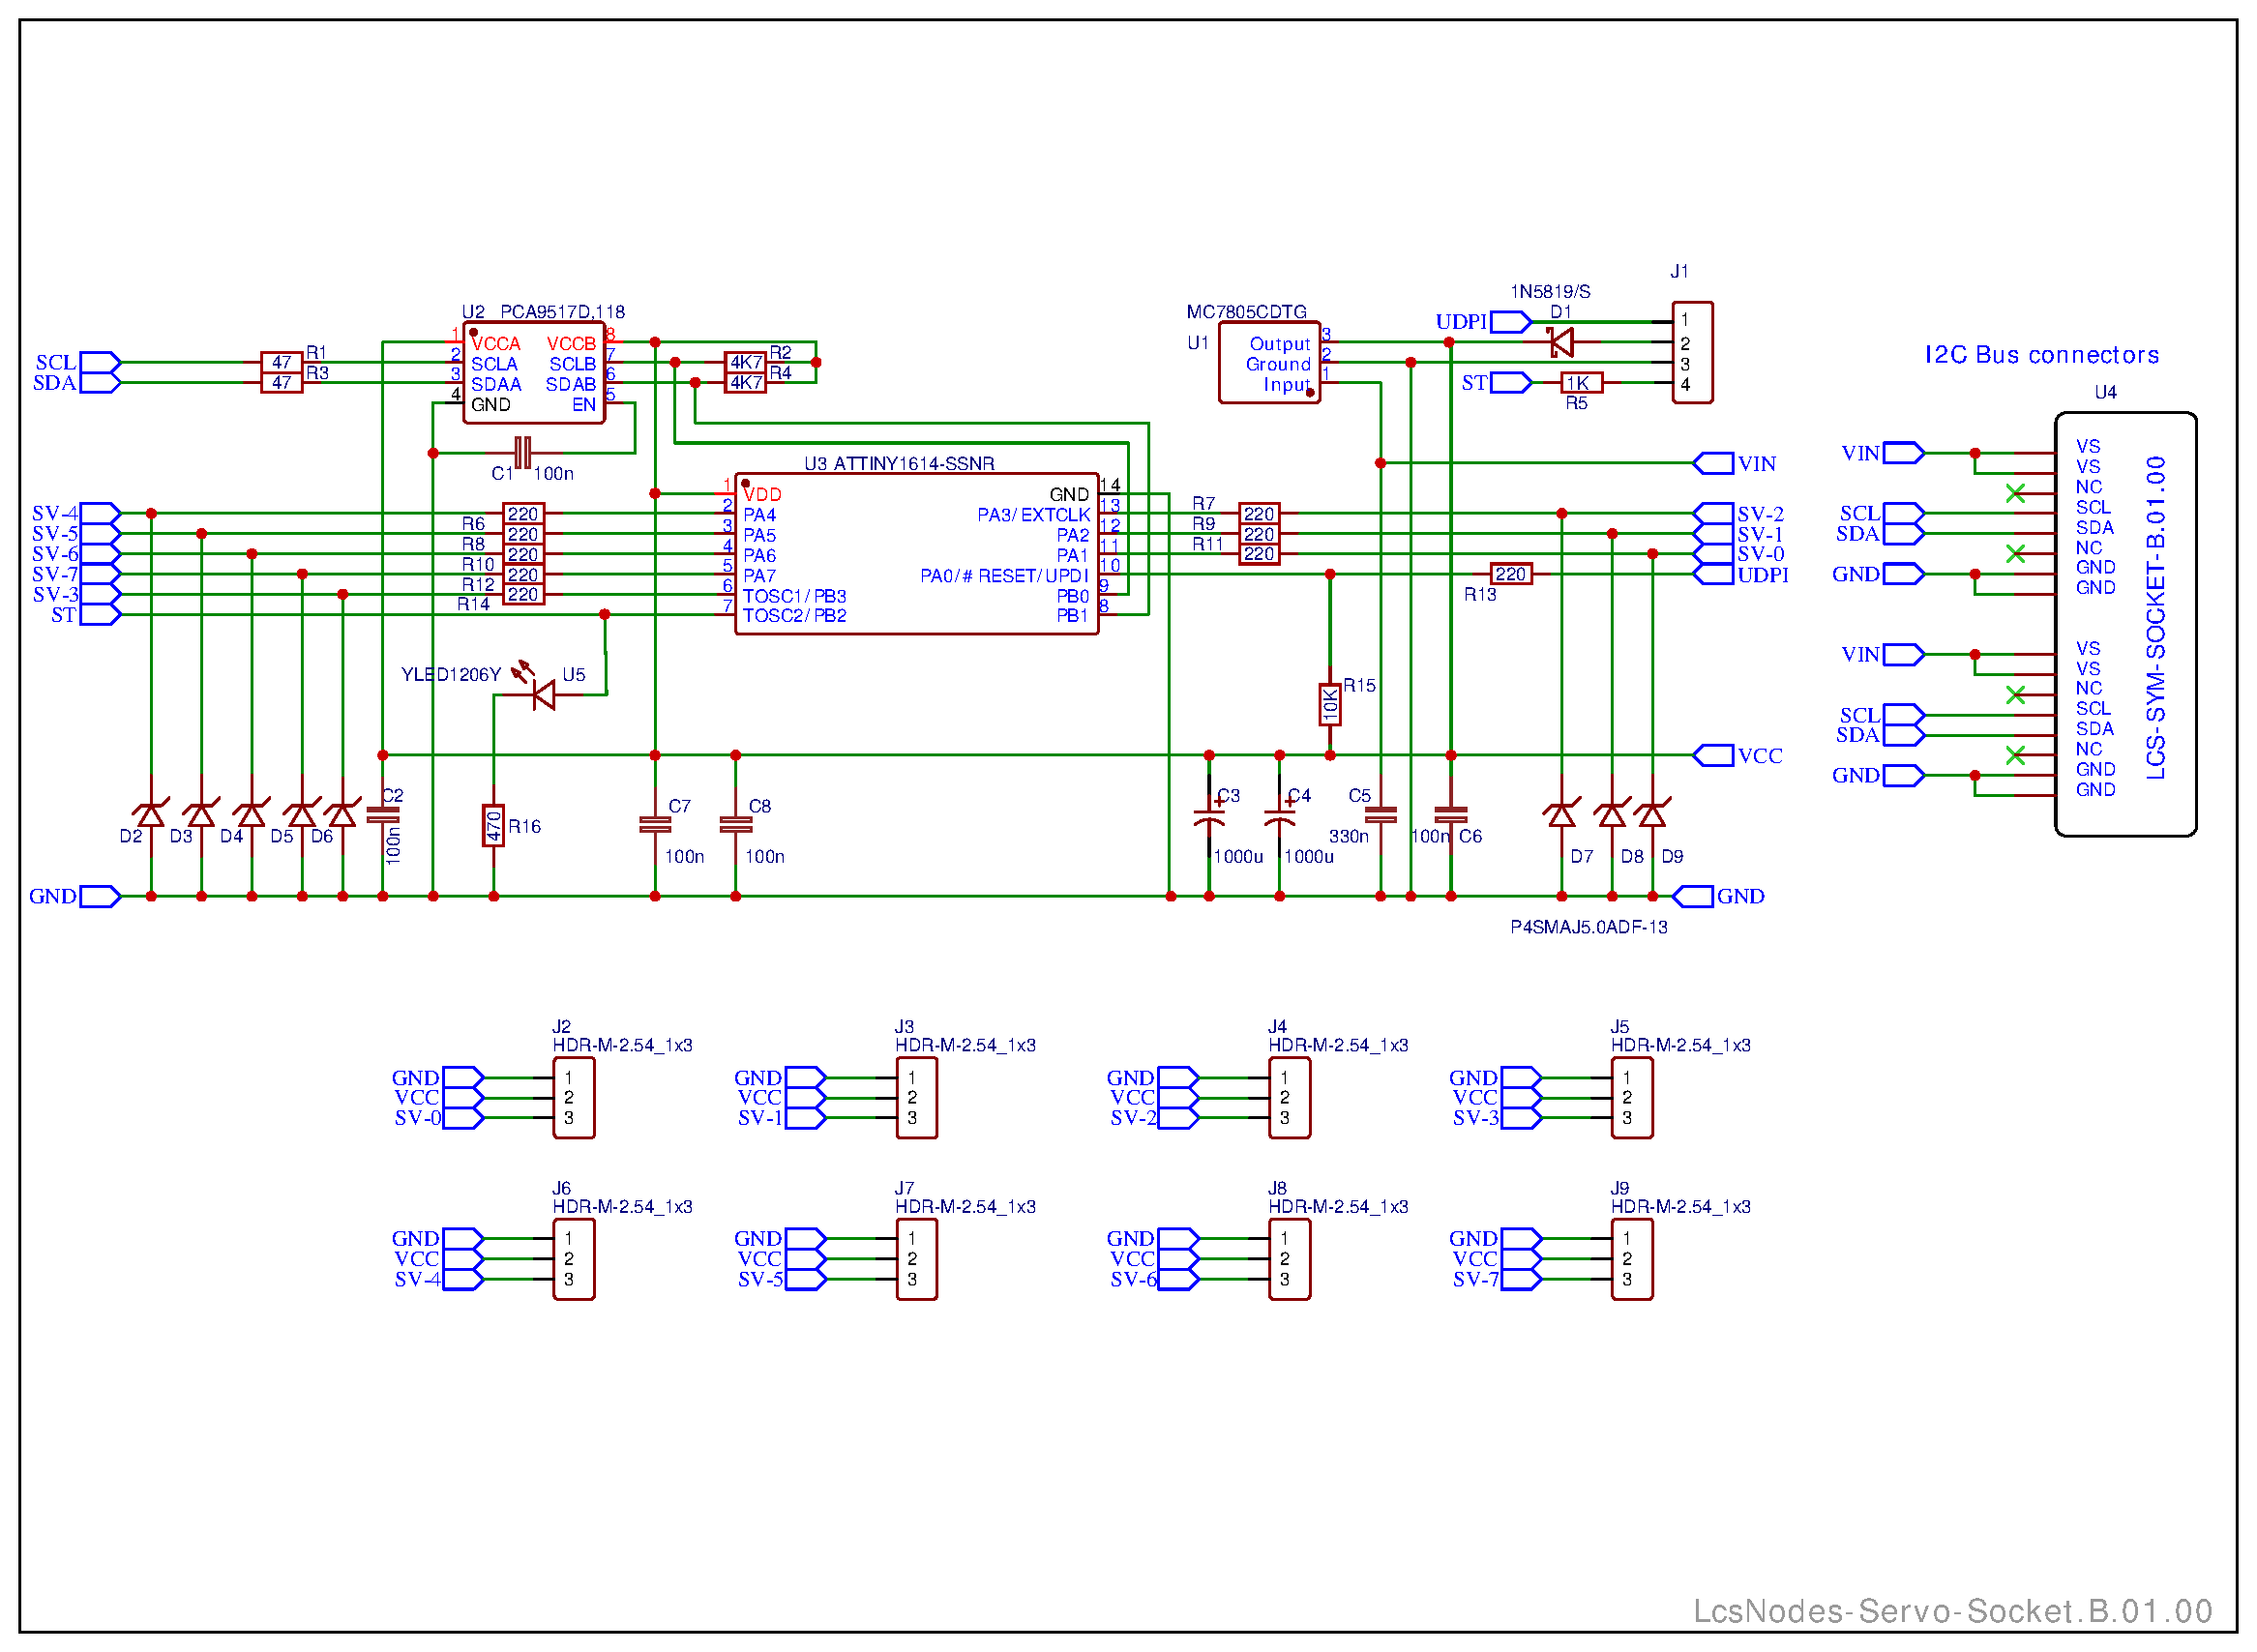
\includegraphics[page=1, width=0.9\textwidth]{./part-extensions/chapter-extension-servos/Schematic_LcsNodes-Servo-Socket-Board-B.01.00.pdf}
\end{figure}
\FloatBarrier


\unnumberedSection{PCB}

\begin{figure}[htbp]
    \centering
    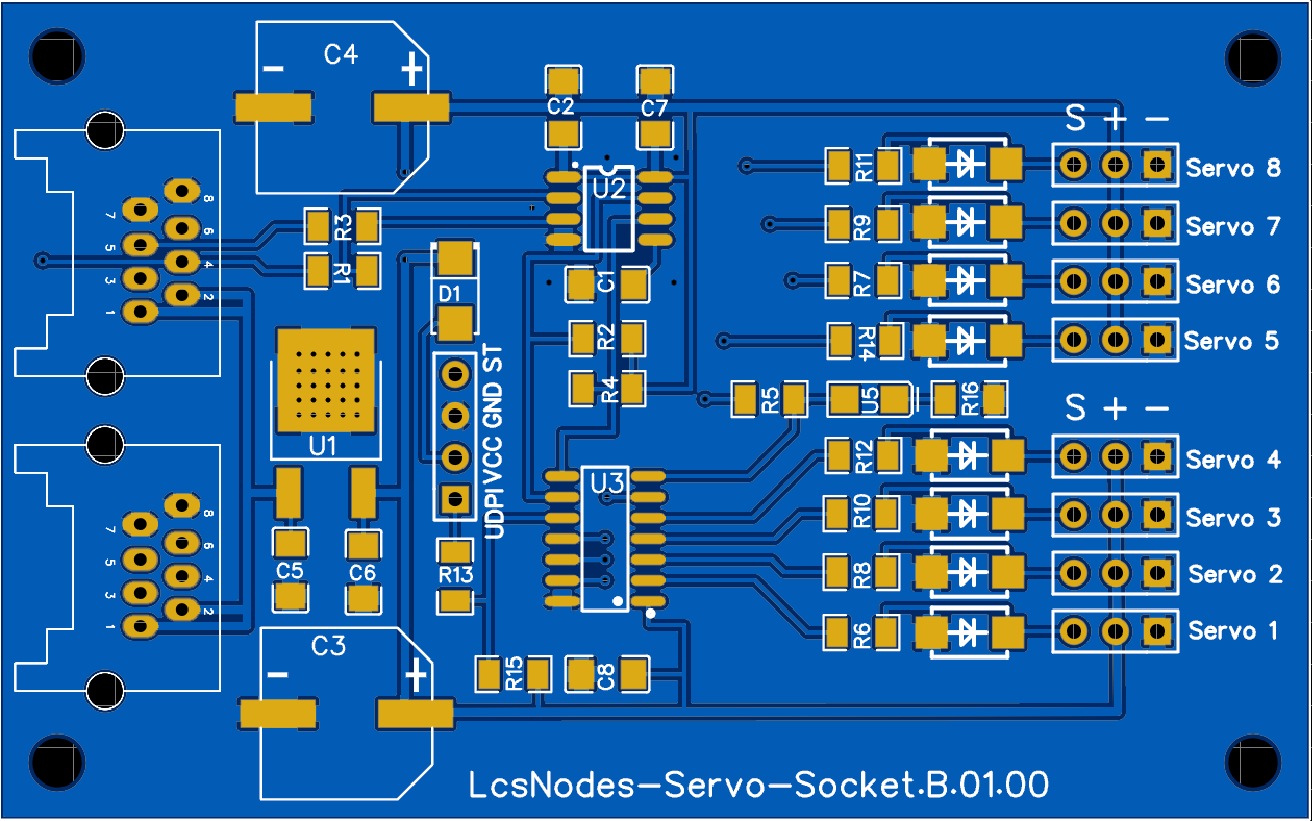
\includegraphics[page=1, width=0.5\textwidth]{./part-extensions/chapter-extension-servos/PCB_LcsNodes-Servo-Socket-Board-B.01.00.pdf}
\end{figure}
\FloatBarrier

\unnumberedSection{Firmware}


\unnumberedSection{Summary}


